\documentclass[10pt,letterpaper,conference]{IEEEtran}

\usepackage{cite}
\usepackage{amsmath}
\usepackage{comment}
%\usepackage{times}
\usepackage{epsfig}
\usepackage{url}
\usepackage{multirow}

\textheight 688pt

\begin{document}
\title{Device-Architecture Co-Optimization of STT-RAM Caches for Embedded Applications\vspace{-10pt}}
%\author{Cong Xu\dag, Xiaochun Zhu\dag\ddag, Dimin Niu\dag, Yuan Xie\dag, Seung H. Kang\dag\ddag\\
%\dag Department of Computer Science and Engineering, Pennsylvania State University\\
%\ddag Emerging Memory Technology Group, Qualcomm Incorpotation\vspace{-15pt}}

\maketitle

\begin{abstract}

Spin-transfer torque random access memory (STT-RAM) is a fast, scalable, durable non-volatile memory which can be embedded into standard CMOS process. A wide range of write speeds from $1ns$ to $100ns$ have been reported for STT-RAM. The switching current of magnetic tunnel junction (MTJ) that is the basic building block of STT-RAM is inversely proportional to the write pulse width. In this work, we provide a detailed methodology to design STT-RAM for different optimization goals such as read performance, write performance and write energy by leveraging the trade-off between write current and write time of MTJ. We take the typical in-plane MTJ and advanced perpendicular MTJ (PMTJ) as our optimization targets. Our study shows that the reducing write pulse width will harm read latency and energy. While "sweet spots" of write pulse width which minimize the write energy or write latency of STT-RAM caches may exist, depending on MTJ species, STT-RAM capacity and I/O width. The simulation results indicate that by utilizing PMTJ, the optimized STT-RAM can compete against SRAM and DRAM as universal memory replacement in low power embedded system.

\end{abstract} 
%\section{Introduction} \label{sec:intro}

Universal memory that provides fast random access, high storage density, and non-volatility within one memory technology becomes possible thanks to the emergence of various new non-volatile memory~(NVM) technologies, such as spin-torque-transfer random-access memory~(STT-RAM, or MRAM), phase-change random-access memory~(PCRAM), and resistive random-access memory~(ReRAM). As the ultimate
goal of these NVM research is to devise a universal memory that could work across multiple layers of the memory hierarchy, each of these emerging NVM technologies has to supply a wide design space that covers a spectrum from highly latency-optimized microprocessor caches to highly density-optimized secondary storage. Among the emerging NVM technologies, STT-RAM seems to be one of the most promising candidates that has the potential to meet all the requirement of universal memory~\cite{STTRAM:Review10B,STTRAM:Review10A}.

STT-RAM was invented as the second generation of Magnetic RAM (MRAM)~\cite{STTRAM:IEDM05} to conquer the two major problems for conventional MRAM: high write energy and poor scalability. Conventional MRAM uses the magnetic fields produced by electrical currents
to change the resistance of the MTJ and the required current increases as technology scales down. The major drawback required current However, in STT-RAM, by applying the spin polarized current through the MTJ element to switch the memory states, the required switching current decreases as technology scales down. Thus STT-RAM is projected to scale beyond 20nm technology node even without any material improvement~\cite{STTRAM:Grandis11}. To further reduce switching current and switching time, Perpendicular MTJs (PMTJ) for STT-RAM were developed~\cite{PMTJ:APL06,PMTJ:APL11,PMTJ:Grandis10,PMTJ:Toshiba08,PMTJ:Xiaochun06} to achieve very low switching current while maintaining relative high thermal stability for non-volatility of STT-RAM. To the best of our knowledge, we are the first to explore the design space of such perpendicular STT-RAM in architecture-level research and it's surprised to see the competitive results of PMTJ versus SRAM even as L1 cache replacement.

Experiments have been performed in device-level research in order to operate a MTJ (magnetic tunnel junction) at minimum energy or energy-delay-product~(EDP) by applying varied write pulse width on MTJ. However, the optimal operating write pulse width from cell-level point of view is not necessarily the best operating point from system-level point of view. Normally an STT-RAM memory cell consists of an access transistor in serial with a MTJ. Short write pulse induced large switching current requires large access transistor for providing enough driving current, which consequently brings more circuit design challenges of the STT-RAM prototype. Specifically, it worsens the area, latency, dynamic energy and leakage power of both memory cells and peripheral circuitry.  Thus it's imperative to offer a methodology for system-level analysis of the memory macro to quantitatively address the trade-off of all the metrics of STT-RAM.

In this work, we implement a system-level performance, energy, and area model to estimate the impact of different write pulse width on the STT-RAM macro design. We then develop a detailed device-architecture co-optimization methodology to design STT-RAM macro with different optimization goals such as area, read latency/energy, write latency, write energy by leveraging the inherent trade-off of write current and write time of MTJ. The results have potential impact on the guidelines for designing a STT-cache in different memory hierarchical levels with different capacities and different optimization goals.

The rest of the paper is organized as follows: Section~\ref{sec:relate} presents related work. Section~\ref{sec:prelim} discusses the basics of STT-RAM and inherent trade-off of write current and write time of MTJ. Section~\ref{sec:model} provides a system-level modeling of STT-RAM macro. Section~\ref{sec:opt} analyzes the optimization methodology of STT-RAM with different optimization goals. Section~\ref{sec:case} shows a case study of replacing L1 cache with STT-RAM in embedded system. Section~\ref{sec:conclusion} concludes our work.

\begin{comment}
Comment Paragraph
\end{comment} 
%\section{STT-RAM Cache Design Optimization} \label{sec:opt}

\begin{figure}[t]
  \centering
  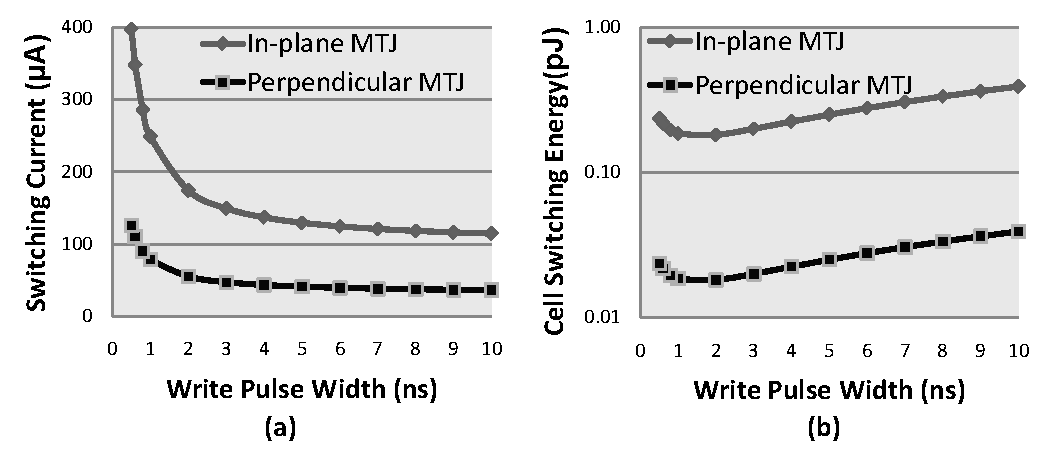
\includegraphics[width=3.5in]{fig/MTJSpec.eps}
  \caption{Representative data curves of in-plane and perpendicular MTJs: (a)Switching current; (b) Cell switching energy.}
  \label{fig:specs}
\end{figure}

\begin{figure*}[t]
  \centering
  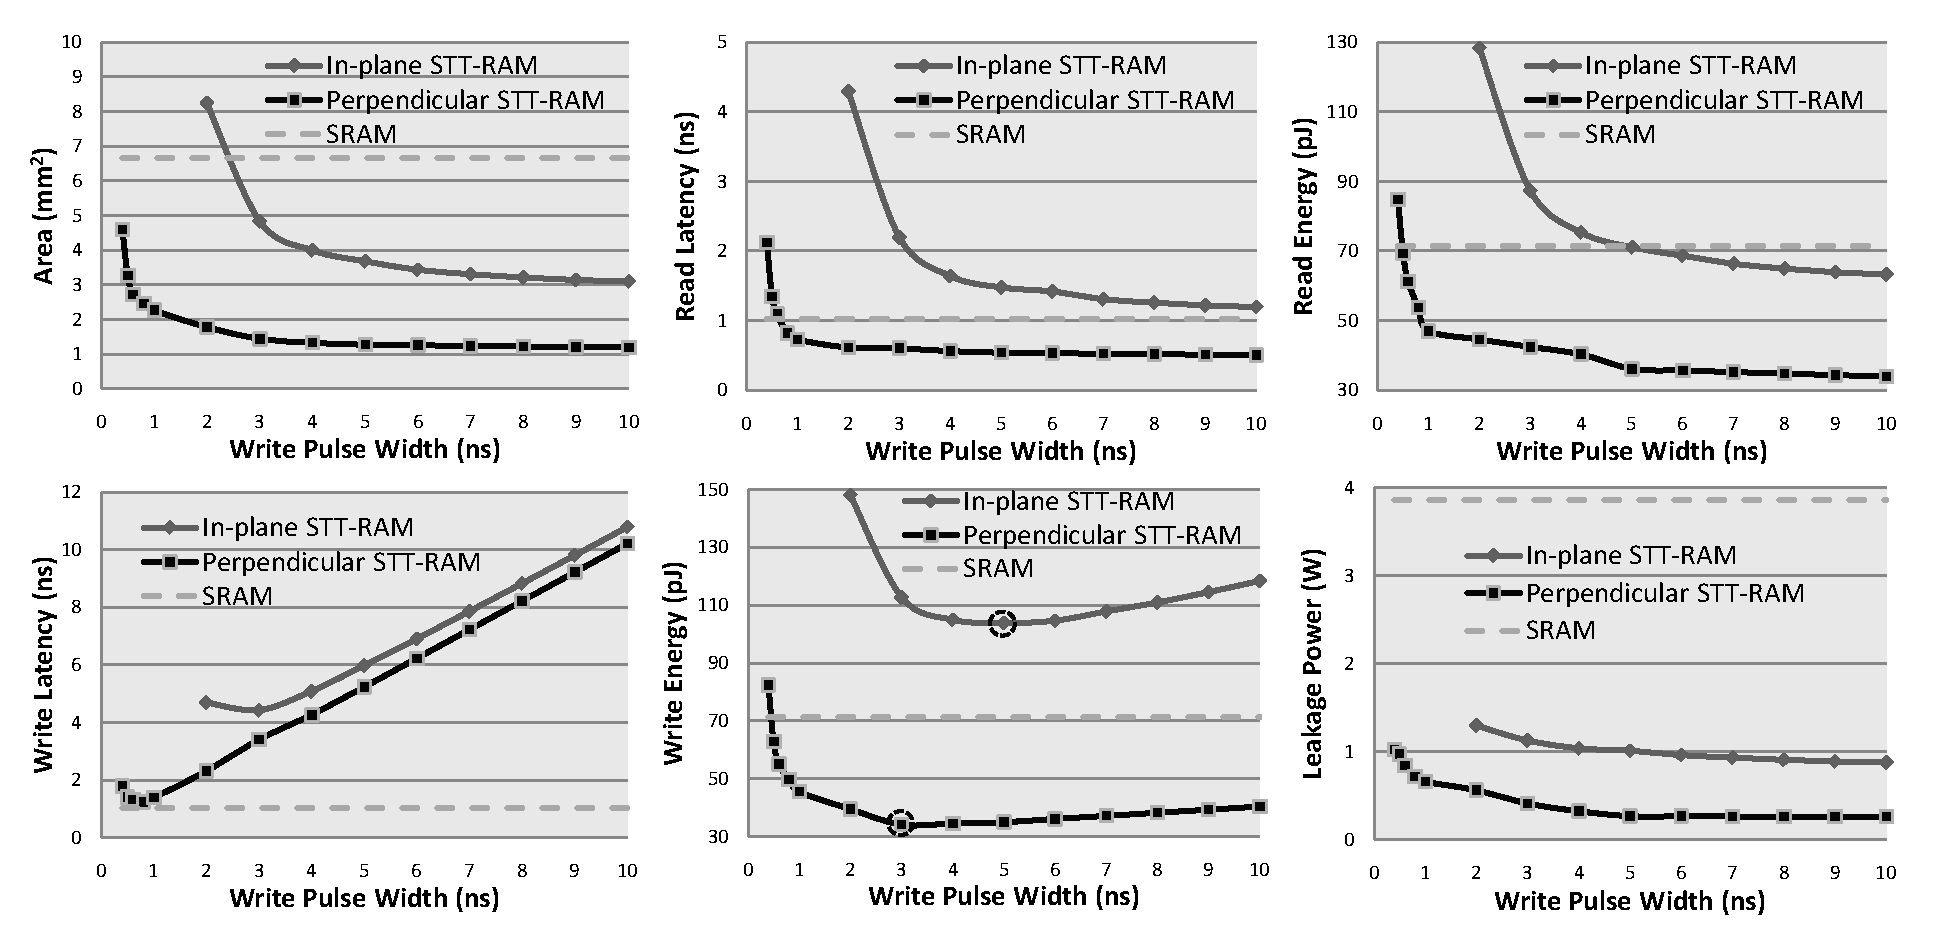
\includegraphics[width=7in]{fig/AllMetrics.eps}
  \caption{Metrics of SRAM and STT-RAM built with in-plane and perpendicular MTJs: (a)Area; (b)Read latency; (c)Read energy; (d)Write latency; (e)Write energy; (f)Leakage power.}
  \label{fig:metrics}
\end{figure*}

\begin{figure}[t]
  \centering
  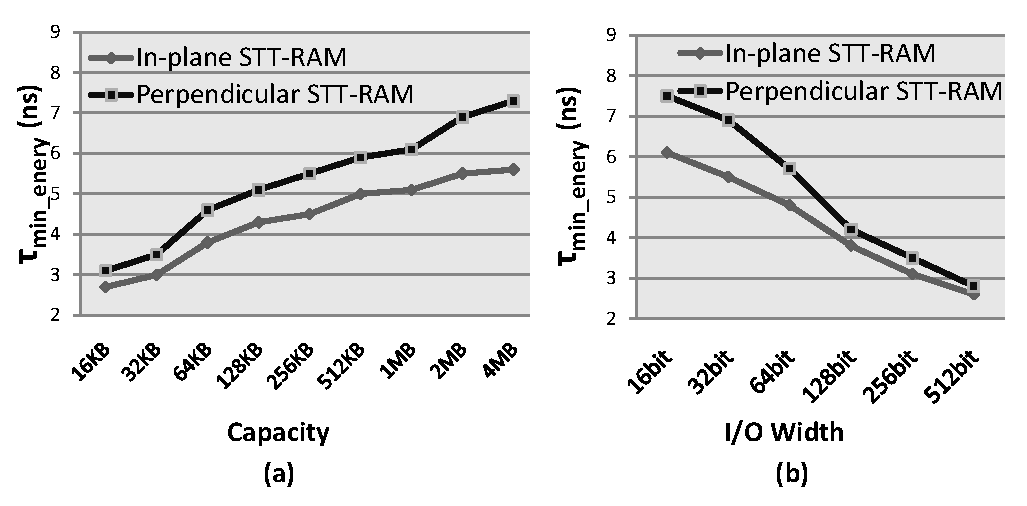
\includegraphics[width=3in]{fig/MinEnergy.eps}
  \caption{Dependence of $\tau_{min\_energy}$ on STT-RAM Macro Capacity.}
  \label{fig:minenergy}
\end{figure}
%\section{Conclusion} \label{sec:conclusion}

In this paper, we analyze the impact of write pulse width on area, performance, and energy of STT-RAM array and develop a methodology for device-architecture co-design of STT-RAM based caches with different optimization goals. We take both near-commercialized in-plane MTJ and advanced PMTJ as optimization targets. Our study shows that for a given MTJ spec the quality of STT-RAM macro strongly depends on the write pulse width. In general, reducing write pulse width will harm area, read operation and leakage and these metrics were exacerbated when the write pulse is shorter than some certain width in processional mode. While write latency/energy is not a non-monotonic function of write pulse width. Therefore it's important to find the optimal write pulse width for minimum write latency or energy. We combine the write pulse width optimization with other architectural techniques to design STT-RAM macro as DRAM or SRAM replacement. A $64MB$ STT-RAM chip design spectrum was demonstrated as potential replacement in low power embedded system. Three STT-RAM caches are verified as L1 cache replacement in an embedded system and the simulation results show that by utilizing advanced PMTJ STT-RAM based L1 cache can outperform SRAM in system performance and energy separately or even simultaneously. 

\bibliographystyle{IEEEtran}
\bibliography{bib/cacti,bib/mram,bib/spintronic,bib/sttram}

\end{document} 